\begin{enumerate}[label=\thesubsection.\arabic*, ref=\thesubsection.\theenumi]
\item The normal form of the equation of a line is
\begin{align}
	\vec{n}^{\top}\vec{x} = c
	\label{eq:EE26BTECH11229-normal-form}
\end{align}
The same form represents a plane when $\vec{x}$ and $\vec{n}$ are $3$-dimensional vectors.
\item The distance between the parallel planes $\vec{n}^{\top}\vec{x} = c_1$ and $\vec{n}^{\top}\vec{x} = c_2$ is
\begin{align}
	d = \frac{\abs{c_2 - c_1}}{\norm{\vec{n}}}
	\label{eq:EE26BTECH11229-plane-dist}
\end{align}
\solution
The point $\vec{x}_1 = \frac{c_1}{\norm{\vec{n}}^2}\vec{n}$ lies on the first plane, from \eqref{eq:EE26BTECH11229-normal-form}. Moving along $\vec{n}$, $\vec{x}_1 + t\vec{n}$ lies on the second plane if
\begin{align}
	\vec{n}^{\top}\brak{\vec{x}_1 + t\vec{n}} = c_2
	\implies c_1 + t\norm{\vec{n}}^2 = c_2
	\implies t = \frac{c_2 - c_1}{\norm{\vec{n}}^2}
\end{align}
The distance is $\abs{t}\norm{\vec{n}}$, yielding \eqref{eq:EE26BTECH11229-plane-dist}.
\item For a square matrix $\vec{A}$ of order $n$,
\begin{align}
	\vec{A}\,\text{adj}\brak{\vec{A}} = \mydet{\vec{A}}\vec{I}
	\label{eq:EE26BTECH11229-adj}
\end{align}
\item (Trace of a Matrix) Let $\vec{A} \in \mathbb{R}^{n \times n}$ be a square matrix with eigenvalues $\lambda_1, \lambda_2, \ldots, \lambda_n$. Then,
\begin{align}
	\sum_{i=1}^{n}\lambda_i = \sum_{i=1}^{n}a_{ii} = \text{tr}\brak{\vec{A}}
	\label{eq:EE26BTECH11229-trace}
\end{align}
\item The probability mass function (PMF) of the outcome $X$ of a fair die is
\begin{align}
	p_X\brak{n} = \begin{cases}
		\frac{1}{6}, & 1 \le n \le 6
		\\
		0, & \text{otherwise}
	\end{cases}
	\label{eq:EE26BTECH11229-die-pmf}
\end{align}
The probability of an event $E$ is
\begin{align}
	\pr{E} = \sum_{n \in E}p_X\brak{n}
	\label{eq:EE26BTECH11229-event-pmf}
\end{align}
\item The events $A$ and $B$ are independent if and only if
\begin{align}
	\pr{AB} = \pr{A}\pr{B}
	\label{eq:EE26BTECH11229-indep}
\end{align}
\item (Continuity) A real-valued function $f\brak{x}$ is continuous at $x = x_0$ if and only if
\begin{align}
	\lim_{x \to x_0^-}f\brak{x} = \lim_{x \to x_0^+}f\brak{x} = f\brak{x_0}
	\label{eq:EE26BTECH11229-continuity}
\end{align}
\item (Differentiability) A function $f\brak{x}$ is differentiable at $x = x_0$ if
\begin{align}
	f^{\prime}\brak{x_0^-} = \lim_{h \to 0^-}\frac{f\brak{x_0 + h} - f\brak{x_0}}{h}
	= \lim_{h \to 0^+}\frac{f\brak{x_0 + h} - f\brak{x_0}}{h} = f^{\prime}\brak{x_0^+}
	\label{eq:EE26BTECH11229-diff-def}
\end{align}
\item If $f\brak{x}$ is differentiable at $x = x_0$, it must necessarily be continuous at $x = x_0$.
\\
\solution
\begin{align}
	\lim_{x \to x_0}\sbrak{f\brak{x} - f\brak{x_0}}
	= \lim_{x \to x_0}\sbrak{\frac{f\brak{x} - f\brak{x_0}}{x - x_0}\brak{x - x_0}}
	= f^{\prime}\brak{x_0}\cdot 0 = 0
	\label{eq:EE26BTECH11229-diff-cont}
\end{align}
\item (Piecewise Boundary Conditions at $x = a$) Consider a function defined by differentiable branches $f_1\brak{x}$ and $f_2\brak{x}$,
\begin{align}
	f\brak{x} = \begin{cases}
		f_1\brak{x}, & x \le a
		\\
		f_2\brak{x}, & x > a
	\end{cases}
\end{align}
For $f\brak{x}$ to be continuous at $x = a$,
\begin{align}
	\lim_{x \to a^-}f_1\brak{x} = \lim_{x \to a^+}f_2\brak{x} \implies f_1\brak{a} = f_2\brak{a}
	\label{eq:EE26BTECH11229-piecewise-cont}
\end{align}
For $f\brak{x}$ to be differentiable at $x = a$, the one-sided derivatives must coincide,
\begin{align}
	f_1^{\prime}\brak{a} = f_2^{\prime}\brak{a}
	\label{eq:EE26BTECH11229-piecewise-diff}
\end{align}
\item (Newton-Raphson Method) For a real-valued differentiable function $g\brak{x}$, the root of $g\brak{x} = 0$ is iteratively approximated using the first-order Taylor series expansion about the current estimate $x_n$, which gives the difference equation
\begin{align}
	x_{n+1} = x_n - \frac{g\brak{x_n}}{g^{\prime}\brak{x_n}}
	\label{eq:EE26BTECH11229-newton}
\end{align}
\solution
The first-order Taylor series of $g\brak{x}$ about $x_n$ is
\begin{align}
	g\brak{x} \approx g\brak{x_n} + g^{\prime}\brak{x_n}\brak{x - x_n}
\end{align}
Equating the right side to zero and calling the solution $x_{n+1}$ yields \eqref{eq:EE26BTECH11229-newton}. If $x_n \to x^*$, then $x^* = x^* - \frac{g\brak{x^*}}{g^{\prime}\brak{x^*}}$, so $g\brak{x^*} = 0$, that is, the limit is a root of $g\brak{x}$.
\item For a quadratic equation $g\brak{x} = ax^2 + bx + c = 0$, we have $g^{\prime}\brak{x} = 2ax + b$, and the difference equation in \eqref{eq:EE26BTECH11229-newton} becomes
\begin{align}
	x_{n+1} = x_n - \frac{ax_n^2 + bx_n + c}{2ax_n + b} = \frac{ax_n^2 - c}{2ax_n + b}
	\label{eq:EE26BTECH11229-newton-quad}
\end{align}
which converges to the root nearest to $x_0$, provided $2ax_0 + b \neq 0$.
\item (Rolle's Theorem) If $f\brak{x}$ is continuous on $\sbrak{a, b}$, differentiable on $\brak{a, b}$ and $f\brak{a} = f\brak{b}$, then there exists $c \in \brak{a, b}$ such that
\begin{align}
	f^{\prime}\brak{c} = 0
	\label{eq:EE26BTECH11229-rolle}
\end{align}
\item If $f^{\prime}\brak{x} > 0$ for all $x$ in an interval, then $f\brak{x}$ is strictly increasing on that interval.
\label{eq:EE26BTECH11229-increasing}

\item (Trapezoidal Rule) Divide $\sbrak{a, b}$ into $N$ equal sub-intervals of width $h = \frac{b - a}{N}$, with $x_n = a + nh$. Approximating $f\brak{x}$ by a straight line on each sub-interval, the integral is computed by the difference equation
\begin{align}
	I_{n+1} = I_n + \frac{h}{2}\brak{f\brak{x_n} + f\brak{x_{n+1}}}, \quad I_0 = 0
	\label{eq:EE26BTECH11229-trapz}
\end{align}
and
\begin{align}
	\int_{a}^{b}f\brak{x}\, dx \approx I_N
\end{align}
\solution
On $\sbrak{x_n, x_{n+1}}$, the area under the straight line joining $\brak{x_n, f\brak{x_n}}$ and $\brak{x_{n+1}, f\brak{x_{n+1}}}$ is a trapezoid,
\begin{align}
	\int_{x_n}^{x_{n+1}}f\brak{x}\, dx &\approx \frac{x_{n+1} - x_n}{2}\brak{f\brak{x_n} + f\brak{x_{n+1}}}
	\nonumber \\
	&= \frac{h}{2}\brak{f\brak{x_n} + f\brak{x_{n+1}}}
\end{align}
Adding this area to the integral $I_n = \int_{a}^{x_n}f\brak{x}\, dx$ obtained so far yields \eqref{eq:EE26BTECH11229-trapz}. For a twice differentiable $f\brak{x}$, the error is
\begin{align}
	\int_{a}^{b}f\brak{x}\, dx - I_N = -\frac{\brak{b - a}h^2}{12}f^{\prime\prime}\brak{\xi}, \quad \xi \in \brak{a, b}
\end{align}
so it decreases as $h^2$.
\item For a continuous function $f\brak{x}$,
\begin{align}
	\int_{0}^{a}f\brak{x}\, dx = \int_{0}^{a}f\brak{a - x}\, dx
	\label{eq:EE26BTECH11229-prop-int}
\end{align}
\solution
Substituting $x = a - t$, $dx = -dt$, the limits $x = 0, a$ become $t = a, 0$,
\begin{align}
	\int_{0}^{a}f\brak{x}\, dx = -\int_{a}^{0}f\brak{a - t}\, dt = \int_{0}^{a}f\brak{a - t}\, dt
\end{align}
\item Trigonometric identities,
\begin{align}
	\tan\brak{\pi - x} = -\tan x, \quad \sec\brak{\pi - x} = -\sec x
	\label{eq:EE26BTECH11229-trig-pi}
\end{align}
\begin{align}
	\frac{\tan x}{\sec x + \tan x} = \frac{\sin x}{1 + \sin x}, \quad
	\frac{1}{1 + \sin x} = \sec^2 x - \sec x\tan x
	\label{eq:EE26BTECH11229-trig-id}
\end{align}
\solution
Multiplying the numerator and the denominator by $\cos x$ gives the first identity. For the second,
\begin{align}
	\frac{1}{1 + \sin x} = \frac{1 - \sin x}{1 - \sin^2 x} = \frac{1 - \sin x}{\cos^2 x}
\end{align}
which equals $\sec^2 x - \sec x\tan x$.
\item The derivatives of $\tan x$ and $\sec x$ are
\begin{align}
	\frac{d}{dx}\tan x = \sec^2 x, \quad \frac{d}{dx}\sec x = \sec x\tan x
	\label{eq:EE26BTECH11229-deriv-sec}
\end{align}
\item The absolute value is defined as
\begin{align}
	\abs{x - a} = \begin{cases}
		x - a, & x \ge a
		\\
		a - x, & x < a
	\end{cases}
	\label{eq:EE26BTECH11229-abs-def}
\end{align}
\item Two vectors $\vec{u}$ and $\vec{v}$ are perpendicular if and only if
\begin{align}
	\vec{u}^{\top}\vec{v} = 0
	\label{eq:EE26BTECH11229-perp-vec}
\end{align}
\item The area of a triangle with two sides $\vec{u}$ and $\vec{v}$ meeting at a vertex is
\begin{align}
	A = \frac{1}{2}\norm{\vec{u}\times\vec{v}}
	\label{eq:EE26BTECH11229-area-cross}
\end{align}
where, for $\vec{u} = \myvec{u_1 \\ u_2 \\ u_3}$ and $\vec{v} = \myvec{v_1 \\ v_2 \\ v_3}$,
\begin{align}
	\vec{u}\times\vec{v} = \myvec{u_2v_3 - u_3v_2 \\ u_3v_1 - u_1v_3 \\ u_1v_2 - u_2v_1}
\end{align}
\item The mean and the variance of a discrete random variable $X$ with PMF $p_X\brak{n}$ are
\begin{align}
	E\brak{X} = \sum_{n}n\,p_X\brak{n}, \quad
	\text{Var}\brak{X} = \sum_{n}n^2\,p_X\brak{n} - \brak{E\brak{X}}^2
	\label{eq:EE26BTECH11229-mean-var}
\end{align}

\item (Sum of Two Cards Drawn from $\cbrak{1, 3, 5, 7}$)
\begin{itemize}
\item Let $X_1, X_2 \in \cbrak{1, 3, 5, 7}$ be independent discrete uniform random variables representing the numbers on two cards drawn with replacement, each having the PMF
\begin{align}
	p_{X_1}\brak{n} = p_{X_2}\brak{n} = \begin{cases}
		\frac{1}{4}, & n \in \cbrak{1, 3, 5, 7}
		\\
		0, & \text{otherwise}
	\end{cases}
	\label{eq:EE26BTECH11229-pmf-cards}
\end{align}
\item Let $X = X_1 + X_2$ denote their sum. The PMF of $X$ is given by the discrete convolution of $p_{X_1}\brak{n}$ and $p_{X_2}\brak{n}$,
\begin{align}
	p_X\brak{n} = \pr{X_1 + X_2 = n} &= \sum_{k}\pr{X_1 = n - k \mid X_2 = k}p_{X_2}\brak{k}
	\\
	&= \sum_{k}p_{X_1}\brak{n - k}p_{X_2}\brak{k} = p_{X_1}\brak{n} * p_{X_2}\brak{n}
	\label{eq:EE26BTECH11229-conv}
\end{align}
\item Substituting \eqref{eq:EE26BTECH11229-pmf-cards} into \eqref{eq:EE26BTECH11229-conv} yields
\begin{align}
	p_X\brak{n} = \begin{cases}
		\frac{1}{16}, & n = 2, 14
		\\
		\frac{2}{16}, & n = 4, 12
		\\
		\frac{3}{16}, & n = 6, 10
		\\
		\frac{4}{16}, & n = 8
		\\
		0, & \text{otherwise}
	\end{cases}
\end{align}
\item The cards are drawn without replacement, so the case $X_1 = X_2$ is not possible. It contributes $\frac{1}{16}$ to $n = 2, 6, 10, 14$, and $\pr{X_1 = X_2} = \frac{1}{4}$. Removing it and normalising by $1 - \frac{1}{4}$ gives the PMF
\begin{align}
	p_X\brak{n} = \begin{cases}
		\frac{1}{6}, & n = 4, 6, 10, 12
		\\
		\frac{1}{3}, & n = 8
		\\
		0, & \text{otherwise}
	\end{cases}
	\label{eq:EE26BTECH11229-pmf-distinct}
\end{align}
\end{itemize}
The following code verifies \eqref{eq:EE26BTECH11229-pmf-distinct} in \figref{fig:EE26BTECH11229-pmf}
\begin{lstlisting}[frame=single, basicstyle=\rmfamily, escapeinside={(*@}{@*)}]
(*@\makebox[\dimexpr\linewidth-2\fboxsep-2\fboxrule\relax][c]{codes/PMF.py}@*)
\end{lstlisting}
\begin{figure}[H]
    \centering
    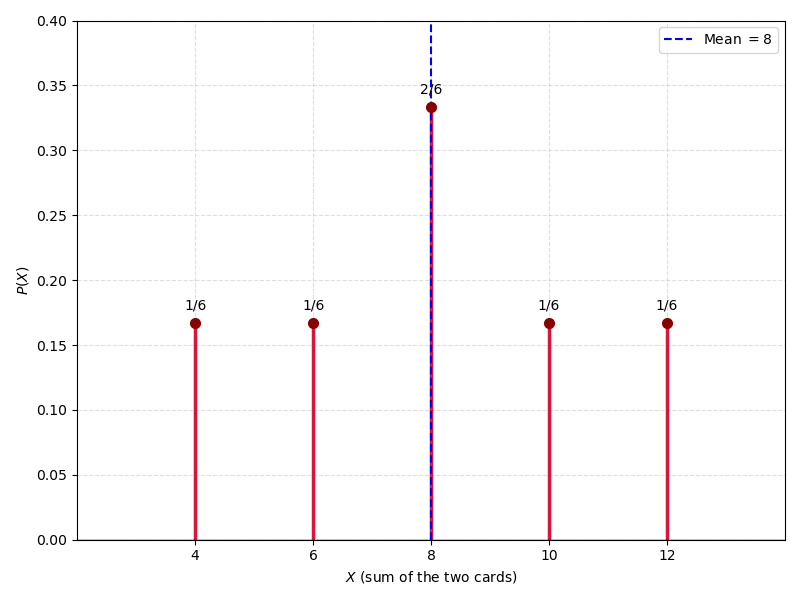
\includegraphics[width=0.75\linewidth]{figs/PMF.png}
    \caption{Probability mass function}
    \label{fig:EE26BTECH11229-pmf}
\end{figure}

\item (Bayes' Theorem) Let $E_1, E_2, \ldots, E_k$ be mutually exclusive events covering the sample space. For an event $A$,
\begin{align}
	\pr{E_i|A} = \frac{\pr{E_i}\pr{A|E_i}}{\sum_{j=1}^{k}\pr{E_j}\pr{A|E_j}}
	\label{eq:EE26BTECH11229-bayes}
\end{align}
\item The value of a determinant does not change if a multiple of one row (or column) is subtracted from another row (or column). A determinant can be expanded along any row or column, using the cofactors of its entries.
\label{eq:EE26BTECH11229-det-props}
\item (System of Linear Equations) The matrix equation
\begin{align}
	\vec{A}\vec{x} = \vec{b}
\end{align}
is consistent if and only if
\begin{align}
	\rank\brak{\vec{A}} = \rank\brak{\sbrak{\vec{A} \mid \vec{b}}} = r
	\label{eq:EE26BTECH11229-consist}
\end{align}
and the solution is unique if $r$ equals the number of unknowns.

\item (Least Squares) If $\vec{A}\vec{x} = \vec{b}$ has more equations than unknowns, the least squares solution minimises
\begin{align}
	\min_{\vec{x}}\norm{\vec{A}\vec{x} - \vec{b}}^2 \implies \vec{x} = \brak{\vec{A}^{\top}\vec{A}}^{-1}\vec{A}^{\top}\vec{b}
	\label{eq:EE26BTECH11229-lstsq}
\end{align}
provided $\rank\brak{\vec{A}}$ equals the number of unknowns. If the system is consistent, the minimum value is zero and $\vec{x}$ is the exact solution.
\solution
Expanding the cost,
\begin{align}
	f\brak{\vec{x}} = \norm{\vec{A}\vec{x} - \vec{b}}^2 = \vec{x}^{\top}\vec{A}^{\top}\vec{A}\vec{x} - 2\vec{b}^{\top}\vec{A}\vec{x} + \vec{b}^{\top}\vec{b}
\end{align}
Setting the gradient to zero,
\begin{align}
	2\vec{A}^{\top}\vec{A}\vec{x} - 2\vec{A}^{\top}\vec{b} = \vec{0} \implies \vec{A}^{\top}\vec{A}\vec{x} = \vec{A}^{\top}\vec{b}
\end{align}
The matrix $\vec{A}^{\top}\vec{A}$ is invertible when $\rank\brak{\vec{A}}$ equals the number of unknowns, which gives \eqref{eq:EE26BTECH11229-lstsq}.

\item The matrix of the points $\vec{A}$, $\vec{B}$, $\vec{C}$ and $\vec{D}$ is $\vec{P} = \myvec{\vec{A} & \vec{B} & \vec{C} & \vec{D}}$, and their direction matrix is
\begin{align}
	\vec{M} = \myvec{\vec{B}-\vec{A} & \vec{C}-\vec{A} & \vec{D}-\vec{A}} = \vec{P}\myvec{-1 & -1 & -1 \\ 1 & 0 & 0 \\ 0 & 1 & 0 \\ 0 & 0 & 1}
	\label{eq:EE26BTECH11229-coplanar}
\end{align}
The points are coplanar if and only if
\begin{align}
	\rank\brak{\vec{M}} < 3
\end{align}
that is, the determinant of $\vec{M}$ is zero.
\item The plane through the points $\vec{A}$, $\vec{B}$ and $\vec{C}$ is
\begin{align}
	\vec{x} = \vec{A} + \lambda\brak{\vec{B}-\vec{A}} + \mu\brak{\vec{C}-\vec{A}}, \quad \lambda, \mu \in \mathbb{R}
	\label{eq:EE26BTECH11229-plane-param}
\end{align}
The point of intersection of this plane with the line in \eqref{eq:EE26BTECH11229-line-param} is obtained by solving the linear system for $\lambda$, $\mu$ and $\kappa$, which has a unique solution if the rank of the coefficient matrix is $3$.
\item The parametric form of the equation of a line is
\begin{align}
	\vec{x} = \vec{h} + \kappa\vec{m}
	\label{eq:EE26BTECH11229-line-param}
\end{align}
where $\vec{m}$ is the direction vector, and $\vec{m}^{\top}\vec{n} = 0$ for a normal $\vec{n}$ of the line.
\item (Line-Conic Intersection) The points of intersection of a line $L: \vec{x} = \vec{h} + \kappa\vec{m}$ $\brak{\kappa \in \mathbb{R}}$ with a conic section $\vec{x}^{\top}\vec{V}\vec{x} + 2\vec{u}^{\top}\vec{x} + f = 0$ are given by
\begin{align}
	\vec{x}_i = \vec{h} + \kappa_i\vec{m}
	\label{eq:EE26BTECH11229-line-conic}
\end{align}
where
\begin{align}
	\kappa_i = \frac{-\vec{m}^{\top}\brak{\vec{V}\vec{h} + \vec{u}} \pm \sqrt{\sbrak{\vec{m}^{\top}\brak{\vec{V}\vec{h} + \vec{u}}}^2 - g\brak{\vec{h}}\brak{\vec{m}^{\top}\vec{V}\vec{m}}}}{\vec{m}^{\top}\vec{V}\vec{m}}, \quad i = 1, 2
\end{align}
with $g\brak{\vec{h}} = \vec{h}^{\top}\vec{V}\vec{h} + 2\vec{u}^{\top}\vec{h} + f$.
\item The area enclosed between the curves $y = f\brak{x}$ (upper) and $y = g\brak{x}$ (lower) from $x = a$ to $x = b$ is
\begin{align}
	A = \int_{a}^{b}\sbrak{f\brak{x} - g\brak{x}}\, dx
	\label{eq:EE26BTECH11229-area-curves}
\end{align}
\item A function $f: X \to Y$ is bijective if it is one-one and onto,
\begin{align}
	f\brak{x_1} = f\brak{x_2} \implies x_1 = x_2, \quad \forall y \in Y, \ \exists x \in X \text{ such that } f\brak{x} = y
	\label{eq:EE26BTECH11229-bij}
\end{align}
The inverse of a bijective function is obtained by solving $y = f\brak{x}$ for $x$.
\item The function $f\brak{x} = \frac{ax + b}{cx + d}$ corresponds to the matrix $\vec{M} = \myvec{a & b \\ c & d}$ acting on $\myvec{x \\ 1}$. Composition of such functions corresponds to the matrix product, and the inverse function corresponds to $\vec{M}^{-1}$ when $\mydet{\vec{M}} \neq 0$.
\label{eq:EE26BTECH11229-mobius}
\item (Inverse by Gauss-Jordan Elimination) The inverse of an $n \times n$ matrix $\vec{A}$ exists if and only if $\rank\brak{\vec{A}} = n$. It is obtained by applying elementary row operations to the augmented matrix until the left half becomes the identity,
\begin{align}
	\sbrak{\vec{A} \mid \vec{I}} \xrightarrow{\text{row operations}} \sbrak{\vec{I} \mid \vec{A}^{-1}}
	\label{eq:EE26BTECH11229-gauss-inverse}
\end{align}
and the solution of $\vec{A}\vec{x} = \vec{b}$ is $\vec{x} = \vec{A}^{-1}\vec{b}$.
\solution
Each row operation is multiplication on the left by an elementary matrix. If $\vec{E}$ is the product of the elementary matrices that reduce $\vec{A}$ to $\vec{I}$, then
\begin{align}
	\vec{E}\sbrak{\vec{A} \mid \vec{I}} = \sbrak{\vec{E}\vec{A} \mid \vec{E}} = \sbrak{\vec{I} \mid \vec{E}}
\end{align}
so $\vec{E}\vec{A} = \vec{I}$ and $\vec{E} = \vec{A}^{-1}$.
\item The Laplace transform of a function $g\brak{t}$ is defined as
\begin{align}
	g\brak{t} \system{L} G\brak{s} = \int_{0}^{\infty}e^{-st}g\brak{t}\, dt
	\label{eq:EE26BTECH11229-laplace-def}
\end{align}
The independent variable can have any name, such as $y$.
\item The Laplace transform of the derivative is
\begin{align}
	g^{\prime}\brak{t} \system{L} sG\brak{s} - g\brak{0}
	\label{eq:EE26BTECH11229-laplace-deriv}
\end{align}
\solution
Applying integration by parts, with $u = e^{-st}$ and $dv = g^{\prime}\brak{t}\, dt$,
\begin{align}
	\int_{0}^{\infty}e^{-st}g^{\prime}\brak{t}\, dt = \sbrak{e^{-st}g\brak{t}}_{0}^{\infty} + s\int_{0}^{\infty}e^{-st}g\brak{t}\, dt = -g\brak{0} + sG\brak{s}
\end{align}
\item Multiplication by $t$ corresponds to differentiation with respect to $s$,
\begin{align}
	t\,g\brak{t} \system{L} -\frac{dG\brak{s}}{ds}
	\label{eq:EE26BTECH11229-laplace-tmult}
\end{align}
\solution
Differentiating \eqref{eq:EE26BTECH11229-laplace-def} with respect to $s$,
\begin{align}
	\frac{dG\brak{s}}{ds} = \int_{0}^{\infty}\brak{-t}e^{-st}g\brak{t}\, dt
\end{align}
\item For a non-negative integer $n$,
\begin{align}
	t^n u\brak{t} \system{L} \frac{n!}{s^{n+1}}
	\label{eq:EE26BTECH11229-laplace-power}
\end{align}
\solution
From $u\brak{t} \system{L} \frac{1}{s}$, applying \eqref{eq:EE26BTECH11229-laplace-tmult} $n$ times gives $\brak{-1}^n\frac{d^n}{ds^n}\frac{1}{s} = \frac{n!}{s^{n+1}}$.
\item (Shift Property) For a constant $a$,
\begin{align}
	e^{at}g\brak{t} \system{L} G\brak{s - a}
	\label{eq:EE26BTECH11229-laplace-shift}
\end{align}
\item The Laplace transforms of the cosine and sine functions are
\begin{align}
	\cos\brak{at}u\brak{t} \system{L} \frac{s}{s^2 + a^2}, \quad
	\sin\brak{at}u\brak{t} \system{L} \frac{a}{s^2 + a^2}
	\label{eq:EE26BTECH11229-laplace-sincos}
\end{align}
\item The linear system $\frac{d\vec{x}}{dt} = \vec{M}\vec{x}$ with $\vec{x}\brak{0} = \vec{x}_0$ has the Laplace transform
\begin{align}
	\vec{X}\brak{s} = \brak{s\vec{I} - \vec{M}}^{-1}\vec{x}_0
	\label{eq:EE26BTECH11229-laplace-system}
\end{align}
\solution
Taking the Laplace transform of each row and using \eqref{eq:EE26BTECH11229-laplace-deriv},
\begin{align}
	s\vec{X}\brak{s} - \vec{x}_0 = \vec{M}\vec{X}\brak{s}
	\implies \brak{s\vec{I} - \vec{M}}\vec{X}\brak{s} = \vec{x}_0
\end{align}
\item For a $2 \times 2$ matrix $\vec{M}$, the poles of $\brak{s\vec{I} - \vec{M}}^{-1}$ are the eigenvalues of $\vec{M}$, and
\begin{align}
	\mydet{s\vec{I} - \vec{M}} = s^2 - \text{tr}\brak{\vec{M}}s + \mydet{\vec{M}}
	\label{eq:EE26BTECH11229-char-poly}
\end{align}
The sum of the eigenvalues is $\text{tr}\brak{\vec{M}}$ and their product is $\mydet{\vec{M}}$.
\end{enumerate}
